\documentclass[10pt,t]{beamer}

\usetheme[progressbar=frametitle]{metropolis}

\usepackage{booktabs}
\usepackage{natbib}
\usepackage[scale=2]{ccicons}
\usepackage{lmodern}

\usepackage{pgfplots}
\usepgfplotslibrary{dateplot}

\usepackage{xspace}
\newcommand{\themename}{\textbf{\textsc{metropolis}}\xspace}
\renewcommand\textbullet{\ensuremath{\bullet}}

\usepackage{tikz}
\usetikzlibrary{shapes.geometric, arrows}
\tikzset{font=\scriptsize}
\tikzstyle{startstop} = [rectangle, rounded corners, minimum width=2.7cm,%
minimum height=0.6cm, text centered, draw=black, fill=mLightBrown!50]
\tikzstyle{compute} = [rectangle, minimum width = 2.7cm, minimum height = 0.7cm,%
text centered, draw=black, fill=mLightGreen!40]
\tikzstyle{logic} = [diamond, minimum width = 1.2cm,%
text centered, draw=black, fill=mDarkTeal, text=white]
\tikzstyle{data} = [circle, minimum width=0.5cm,text centered,%
draw=black,fill=white]
\tikzstyle{arrow} = [thick,->,>=stealth]
\tikzstyle{line} = [thick]


%% symbols
\newcommand{\bX}{\mathbf{X}}
\newcommand{\bY}{\mathbf{Y}}
\newcommand{\mat}[1]{\mathbf{#1}}
\renewcommand{\vec}[1]{\boldsymbol{#1}}


\title{Real time prediction of bus arrival}
%\subtitle{}
\date{SET THE DATE, 2016}
\author{Tom Elliott}
\institute{Supervised by Professor Thomas Lumley\\[2em]

\includegraphics[height=1.5cm]{stat-logo.png}}
%Department of Statistics\\University of Auckland}
%\titlegraphic{\hfill
\includegraphics[height=1.5cm]{stat-logo.png}}

\begin{document}

\maketitle



\begin{frame}{Motivation}
  \begin{itemize}[<+->]
  \item ``Bus prediction'' isn't something new

  \item Automatic Vehicle Location (AVL) technologies
    \begin{itemize}
    \item 1964: Hamburg, Germany
    \item Auckland Transport uses GPS --- buses report position periodically
    \item Not perfect: interference etc
    \end{itemize}

  \item AVL based prediction models not that good (at least in Auckland)
    \begin{itemize}
    \item Inputs: AVL, schedule, historical \ldots ?
    \item Several problematic situations: major delays, cancellations, \textbf{loops}
    \end{itemize}
  \end{itemize}

  %\metroset{block=fill}
%  \item \emph{Improved} bus prediction
  % \onslide<+->
  % \begin{block}{Improved Bus Prediction}
  %   \begin{enumerate}[<1->]
  %   \item more robust real-time model
  %   \item improved prediction model: ``real-time'' data
  %   \item arrival time \emph{prediction intervals}, journey planning
  %   \end{enumerate}
  % \end{block}

 % \end{itemize}
\end{frame}


\begin{frame}{Motivation: Example}
  An example of a situation where a loop breaks the current model,
  evidenced by AT's \emph{Track My Bus} app:

  \onslide<2->{Scheduled Arrival stop 5594: 7:24am (counter-clockwise loop)}
  
  \vspace{0.5em}
  \centering
  \includegraphics<3>[width=0.45\textwidth,trim={0 0 0 15cm},clip]{figs/bus-loop-durp1.jpg}
  \includegraphics<4>[width=0.45\textwidth,trim={0 0 0 15cm},clip]{figs/bus-loop-durp2.jpg}

  \begin{overprint}
    \onslide<3>
    \centering
    7:24am
    \onslide<4>
    \centering
    7:26am
  \end{overprint}

\end{frame}




\begin{frame}[fragile]{Overview}
  \begin{enumerate}
    \item General Transit Feed Specification (GTFS)

    \item Recursive Bayesian filtering

    \item Real-time bus models

    \item Predictive models: future arrival times

    \item Making it available to commuters
      \begin{itemize}
      \item Communicating predictive errors, uncertainty
      \item Journey Planning application
      \end{itemize}

  \end{enumerate}
\end{frame}




\section{GTFS}

\begin{frame}{GTFS}

  \begin{itemize}[<+->]
    \item General Transit Feed Specification
      \begin{itemize}
      \item \textbf{Static}: schedule information: trips, routes, shapes,
        schedules
      \item \textbf{Realtime}: GPS location of buses
      \end{itemize}

    \item Developed and standardised by Google and used globally
    \item API provided by Auckland Transport (AT)\\
      \url{https://dev-portal.at.govt.nz}
  \end{itemize}

  \begin{overprint}
    \onslide<4>
    \begin{figure}
      \vspace{-3em}
      \centering
      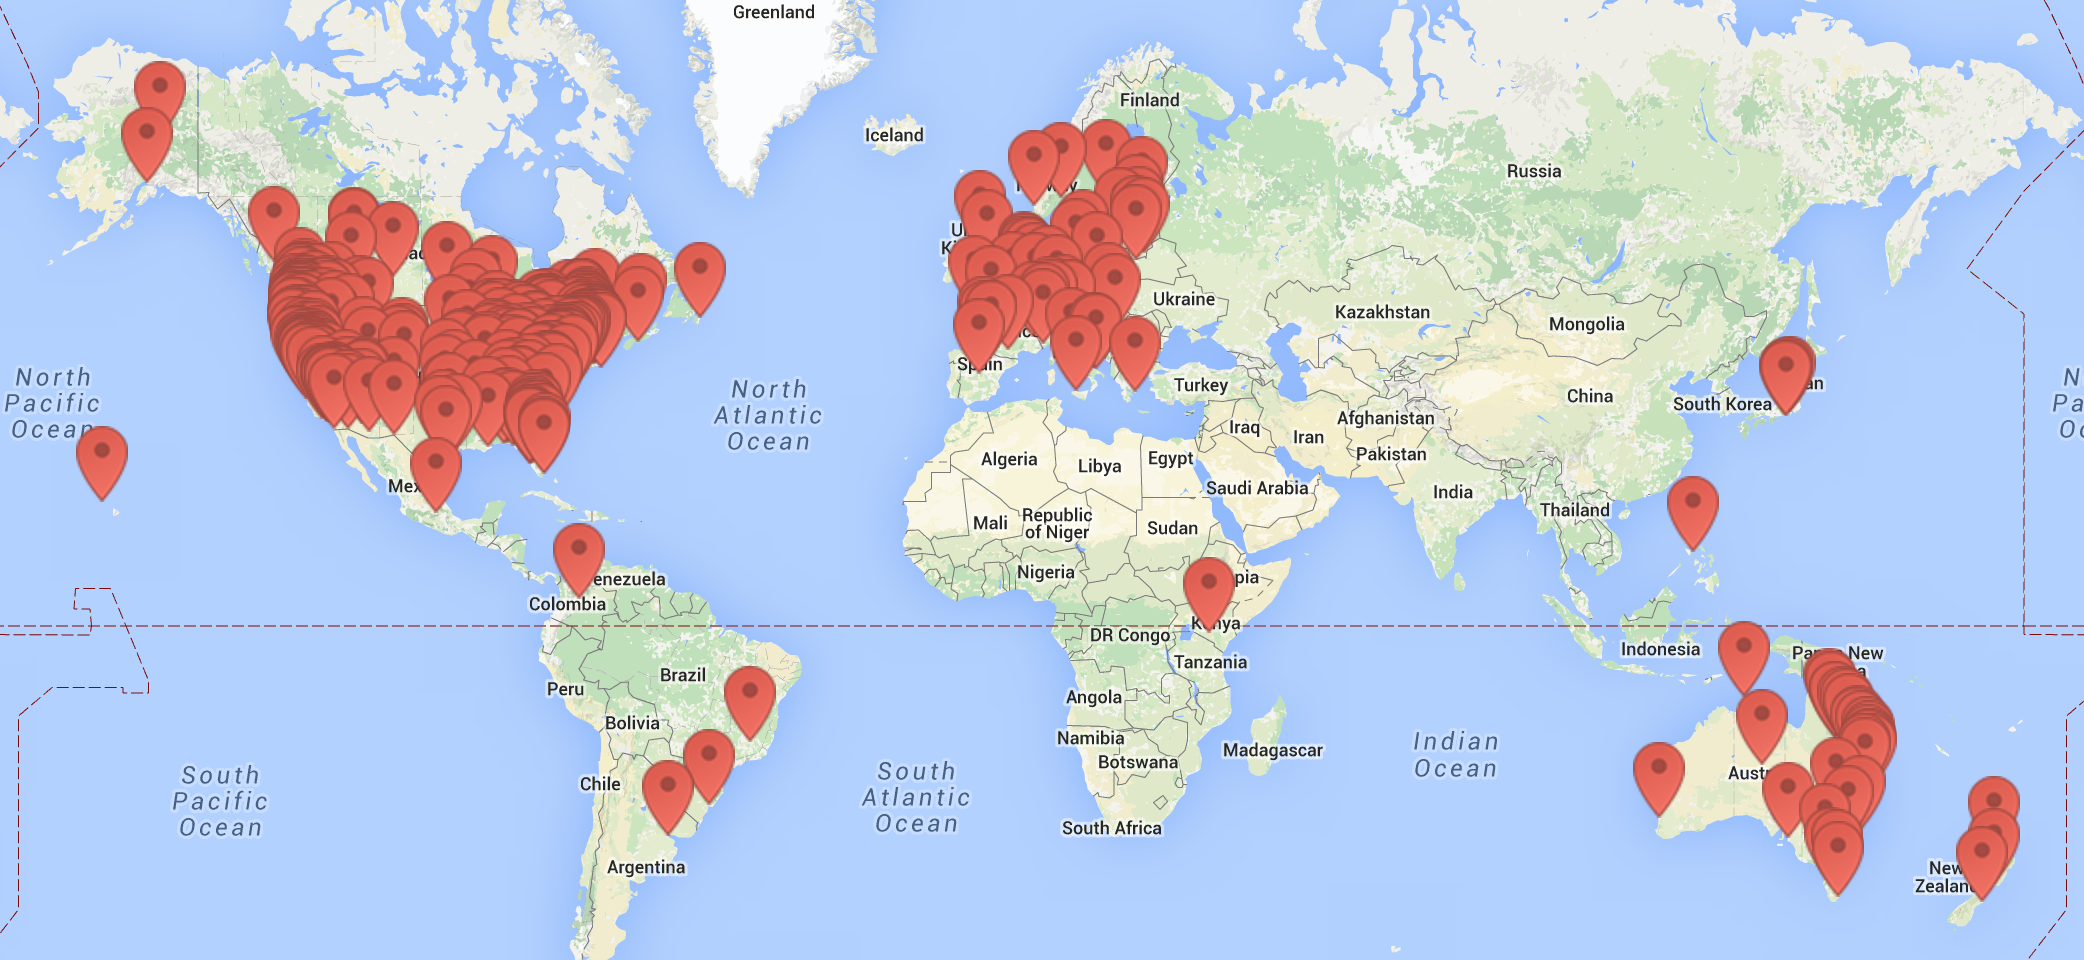
\includegraphics[height=4cm]{gtfs-feeds.png}
      \caption{Global GTFS feeds, \url{http://transitfeeds.com/}}
    \end{figure}
  \end{overprint}

\end{frame}





\section{Recursive Bayesian Filtering}

\begin{frame}{Recursive Bayesian Filtering}
  \onslide<+->
  \begin{itemize}[<+->]
    \item new observations every 30 seconds:
      \begin{equation*}
        \bY_k =
        \begin{bmatrix}
          \phi_k & \lambda_k & t_k
        \end{bmatrix}^T
      \end{equation*}
      $\phi$ = latitude (north/south), $\lambda$ = longitude (east/west)

    \item correspond to unknown and unmeasurable \emph{state}:
      \begin{equation*}
        \bX_k =
        \begin{bmatrix}
          d_k & v_k & \cdots
        \end{bmatrix}^T
      \end{equation*}
      $d$ = distance into trip (m), $v$ = velocity (speed, m/s)

    \item new state \emph{predicted} using previous state, \emph{updated} using latest observation:
      \begin{equation*}
        \bX_k = f(\bX_{k-1}, \bY_k)
      \end{equation*}
  \end{itemize}

\end{frame}


\begin{frame}{Recursive Bayesian Filtering: Kalman Filter I}
  \onslide<+->
  \begin{itemize}%[<+- | alert@+>]
    \item Used in robotics, navigation, tracking, etc.

    \item Several bus tracking/prediction applications\\
      (\cite{wall-dailey:1999}, \cite{dailey:2001}, \cite{cathey-dailey:2003}, \ldots)

    \item Very fast (matrix multiplication) = good for real-time applications
    \end{itemize}


    \begin{enumerate}[<+->]
    \item \textbf{Predict}:
      \begin{equation*}
        \bX_k = \mat{A}_k \bX_{k-1} + \vec{w}_k
      \end{equation*}
      $\mat{A}_k$ depends on $\delta_k$ = time since last observation\\
      $\vec{w}_k$ = Gaussian process noise
    \item \textbf{Update}:
      \begin{equation*}
        \vec{z}_k = \mat{H} \bX_k + \vec{v}_k
      \end{equation*}
      $\mat{H} $ = observation model\\
      $\vec{v}_k$ = Gaussian measurement error\\
      $\vec{z}_k$ = observed data$^\dagger$
    \end{enumerate}

\end{frame}


\begin{frame}{Recursive Bayesian Filtering: Kalman Filter II}
  \onslide<+->
  \begin{itemize}[<+->]
      \item Everything is normal: mean vector and covariance matrix

      \item Cannot compare $\bX_k$ directly to $\bY_k$,
        first estimate $\vec{z}_k$\\
        i.e., given $\bY_k$, where on the route (2D line) is the bus most likely?

      \item Dynamics/transitions specified in matrix $\mat{A}_k$: e.g., 
        \begin{equation*}
          \hat\bX_k = \mat{A}_k \bX_{k-1} = \begin{bmatrix} 1 & \delta_k \\ 0 & 1 \end{bmatrix}
          \begin{bmatrix} d_{k-1} \\ v_{k-1} \end{bmatrix}
        \end{equation*}
        $\hat d_k = d_{k-1} + v_{k-1}\delta_k$
        (Newton's Laws of Motion)

      \item not easy to include complex features: e.g., dwell times

      \item assumes \textbf{multivariate normality} --- stops, loops = multimodal
  \end{itemize}

\end{frame}



\begin{frame}{Recursive Bayesian Filtering: Particle Filter I}
  \onslide<+->
  \begin{itemize}[<+->]
    \item Generalises the Kalman Filter
      
    \item Sample of particles (``imaginary buses'') with state $\bX_k^{(i)}$

    \item \textbf{Predict} step: model particles \emph{individually}:
      \begin{equation*}
        \tilde\bX_k^{(i)} = f(\bX_{k-1}^{(i)}, \sigma_v^2)
      \end{equation*}
      No restrictions on $f$ (except computational)

    \item \textbf{Update} step: weighted resample (importance resampling)
      \begin{equation*}
        w_k^{(i)} = \frac{p(\bY_k | \tilde\bX_k^{(i)})}{\sum_{j=1}^M p(\bY_k | \tilde\bX_k^{(j)})}
      \end{equation*}
      
    \item no intermediate estimation of $\vec{z}_k$

    \item New sample approximates \emph{posterior distribution} of $\bX_k$
  \end{itemize}
\end{frame}


\begin{frame}{Recursive Bayesian Filtering: Particle Filter II}
  \begin{itemize}[<+->]
  \item Likelihood depends on distance between particle ($d_k^{(i)}$) and reported position ($\bY_k$)
  \item Transform particle's distance to coordinate using shape information
    
    \includegraphics[width=0.45\textwidth]{gps-dist2.jpg}
    \includegraphics[width=0.45\textwidth]{gps-dist1.jpg} 
    
  \item Use (Great Circle) distance between two coordinates
  \item No estimation of $\vec{z}_k$ required!
  \end{itemize}
\end{frame}



\begin{frame}{Recursive Bayesian Filtering: Particle Filter III}
  A simple example using only one dimension (distance).

  \onslide<+->
  \begin{itemize}[<+- | alert@+>]
    \item Start with previous state $\bX_{k-1}$
    \item Use model (bus dynamics, dwell times, etc) to predict state $\tilde\bX_{k}$
    \item Add process noise
    \item Get observation $\bY_k$
    \item Compute weights based on distance from observation
    \item Weighted resample to get $\bX_k$
  \end{itemize}
  %\vspace{5cm}
  \begin{overprint}
    \onslide<2>
    \centering
    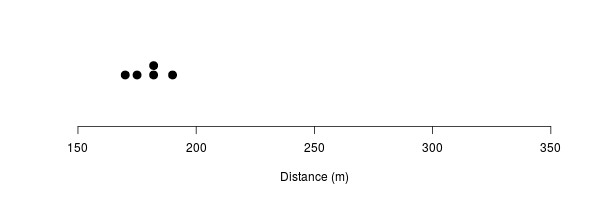
\includegraphics[width=0.8\textwidth]{figs/pf1-frame1.png}
    \onslide<3>
    \centering
    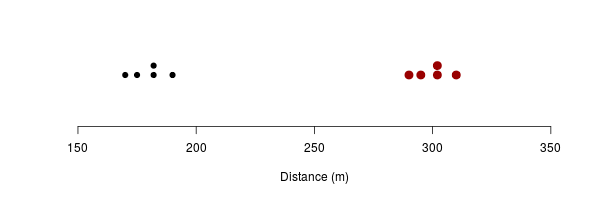
\includegraphics[width=0.8\textwidth]{figs/pf1-frame2.png}
    \onslide<4>
    \centering
    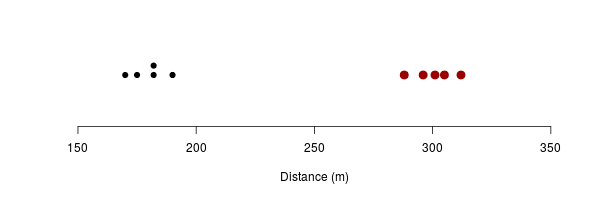
\includegraphics[width=0.8\textwidth]{figs/pf1-frame3.png}
    \onslide<5>
    \centering
    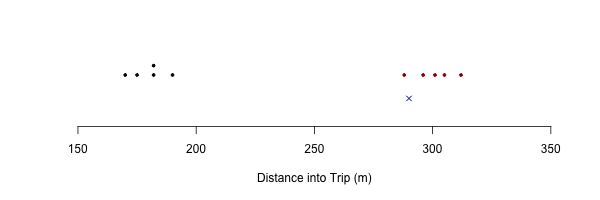
\includegraphics[width=0.8\textwidth]{figs/pf1-frame4.png}
    \onslide<6>
    \centering
    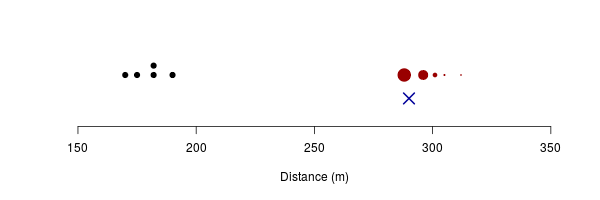
\includegraphics[width=0.8\textwidth]{figs/pf1-frame5.png}
    \onslide<7->
    \centering
    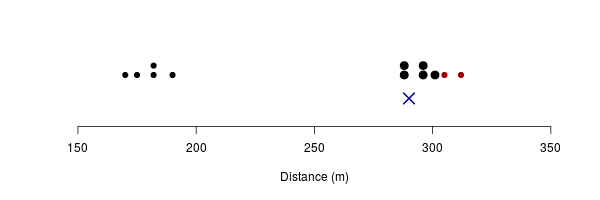
\includegraphics[width=0.8\textwidth]{figs/pf1-frame6.png}
  \end{overprint}
  \onslide<+->
\end{frame}


\section{Real-time Bus Models}

\begin{frame}{Real-time Models I: Bus Behaviour}
  \onslide<+->
  \begin{itemize}[<+->]
  \item Follow motion laws between stops
  \item Stop at bus stop $j$ with probability $\pi_j$
  \item If bus stops:
    \begin{itemize}[<1->]
    \item decelerate and open doors
    \item allow passengers to alight and embark
    \item close doors and accelerate
    \end{itemize}
  \item If bus doesn't stop, do none of the above
  \item Traffic lights: no info (yet) on their locations (in Auckland)
  \end{itemize}
\end{frame}


\begin{frame}{Real-time Bus Models II: Dwell Times}
  \onslide<+->
  \begin{itemize}[<+->]
    \item Dwell time at stop $j = \tau_j$ = \emph{time lost due to stopping}
    \item Given a bus stops \ldots
      
      \begin{itemize}[<1->]
      \item every stop: decelerate, open/close doors, and accelerate: $\gamma$
      \item stop $j$: wait until passengers have alighted/boarded: $\tau_j'$
      \item dwell time: $\tau_j = \gamma + \tau_j'$
      \end{itemize}

    \item Particle filter model
      \begin{itemize}
        \item Include logic in $f$
        \item Does particle (``imaginary bus'') stop?\\
          $p_j^{(i)} \sim \text{Bernoulli}(\pi_j)$, $\tau_j'^{(i)} \sim \mathcal{E}(\mu_\tau)$
        \item dwell time =  $p_j^{(i)} (\gamma + \tau_j'^{(i)})$
        \item multimodal distribution!
      \end{itemize}
    \end{itemize}

  \vspace{-6em}
  \begin{overprint}
    \onslide<3>
    \centering
    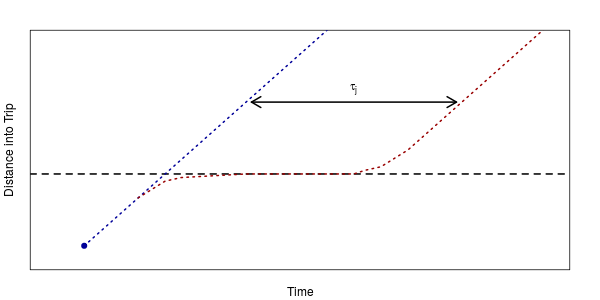
\includegraphics[width=0.8\textwidth]{figs/dwell_time.png}
  \end{overprint}
\end{frame}


\begin{frame}{Real-time Bus Models III}
  Particle Filter model, $\bX_k = f(\bX_{k-1}, \bY_k, \sigma_v, \sigma_y, \ldots)$

  \vspace{0.5cm}
  \begin{tikzpicture}[node distance=1.4cm]
    \node (start) [startstop] {Previous State, $\bX_{k-1}$};
    \node (move) [compute, below of=start,align=center] {Add noise, $\sigma_v$\\ Move Forward};
    \node (stateEst) [startstop, below of=move] {Estimated State, $\tilde\bX_k$};
    \node (resample) [compute, below of=stateEst,align=center] %
    {Compute likelihood, $\sigma_y$\\Weighted Resample};
    \node (end) [startstop, below of=resample] {Final State, $\bX_k$};

    \node (data) [data, right of=resample, xshift=1cm] {$\bY_k$};

    \onslide<2->{\node (passStop) [logic, right of=move, xshift=1.5cm] {\tiny Pass stop?};
    \node (arrival) [compute, right of=passStop, xshift=1.5cm, align=center]%
      {Get arrival time\\ Sample $p \sim \text{Bern}(\pi)$\\%
      Sample $\tau \sim \mathcal{E}(\mu_\tau)$};
    \node (remaining) [logic, right of=arrival, xshift=1.5cm] {\tiny Time left?};
    \node (moveForward) [compute, above of=arrival, align=center]%
      {Get departure time\\Move forward};
    \node (stopped) [compute, below of=arrival] {Position at stop};
    }

    \draw [arrow] (start) -- (move);
    \draw [arrow] (stateEst) -- (resample);
    \draw [arrow] (data) -- (resample);
    \draw [arrow] (resample) -- (end);
    \onslide<1>\draw [arrow] (move) -- (stateEst);
    \onslide<2->\draw [arrow] (move) -- (passStop);

    \draw [arrow] (passStop) -- node[anchor=south] {yes} (arrival);
    \draw [arrow] (arrival) -- (remaining);
    \draw [arrow] (remaining) |- node[anchor=west] {yes} (moveForward);
    \draw [arrow] (moveForward) -| (passStop);
    \draw [arrow] (remaining) |- node[anchor=west] {no} (stopped);
    \draw [arrow] (stopped) -- coordinate[midway] (toEst) (stateEst);
    \draw [line] (passStop) -- node[anchor=west] {no} (toEst);
  \end{tikzpicture}
\end{frame}


\begin{frame}{Example}
  \begin{itemize}
    \item Applied to data collected from a bus route
    \item Non-informative priors (speed, dwell times, stopping probabilities)
    \item \emph{Always} a small probability of not moving (e.g., traffic lights)
  \end{itemize}
\end{frame}

{ % all template changes are local to this group.
    \setbeamercolor{background canvas}{bg=white}
    \begin{frame}[plain]
        \begin{tikzpicture}[remember picture,overlay]
            \node[at=(current page.center)] {
                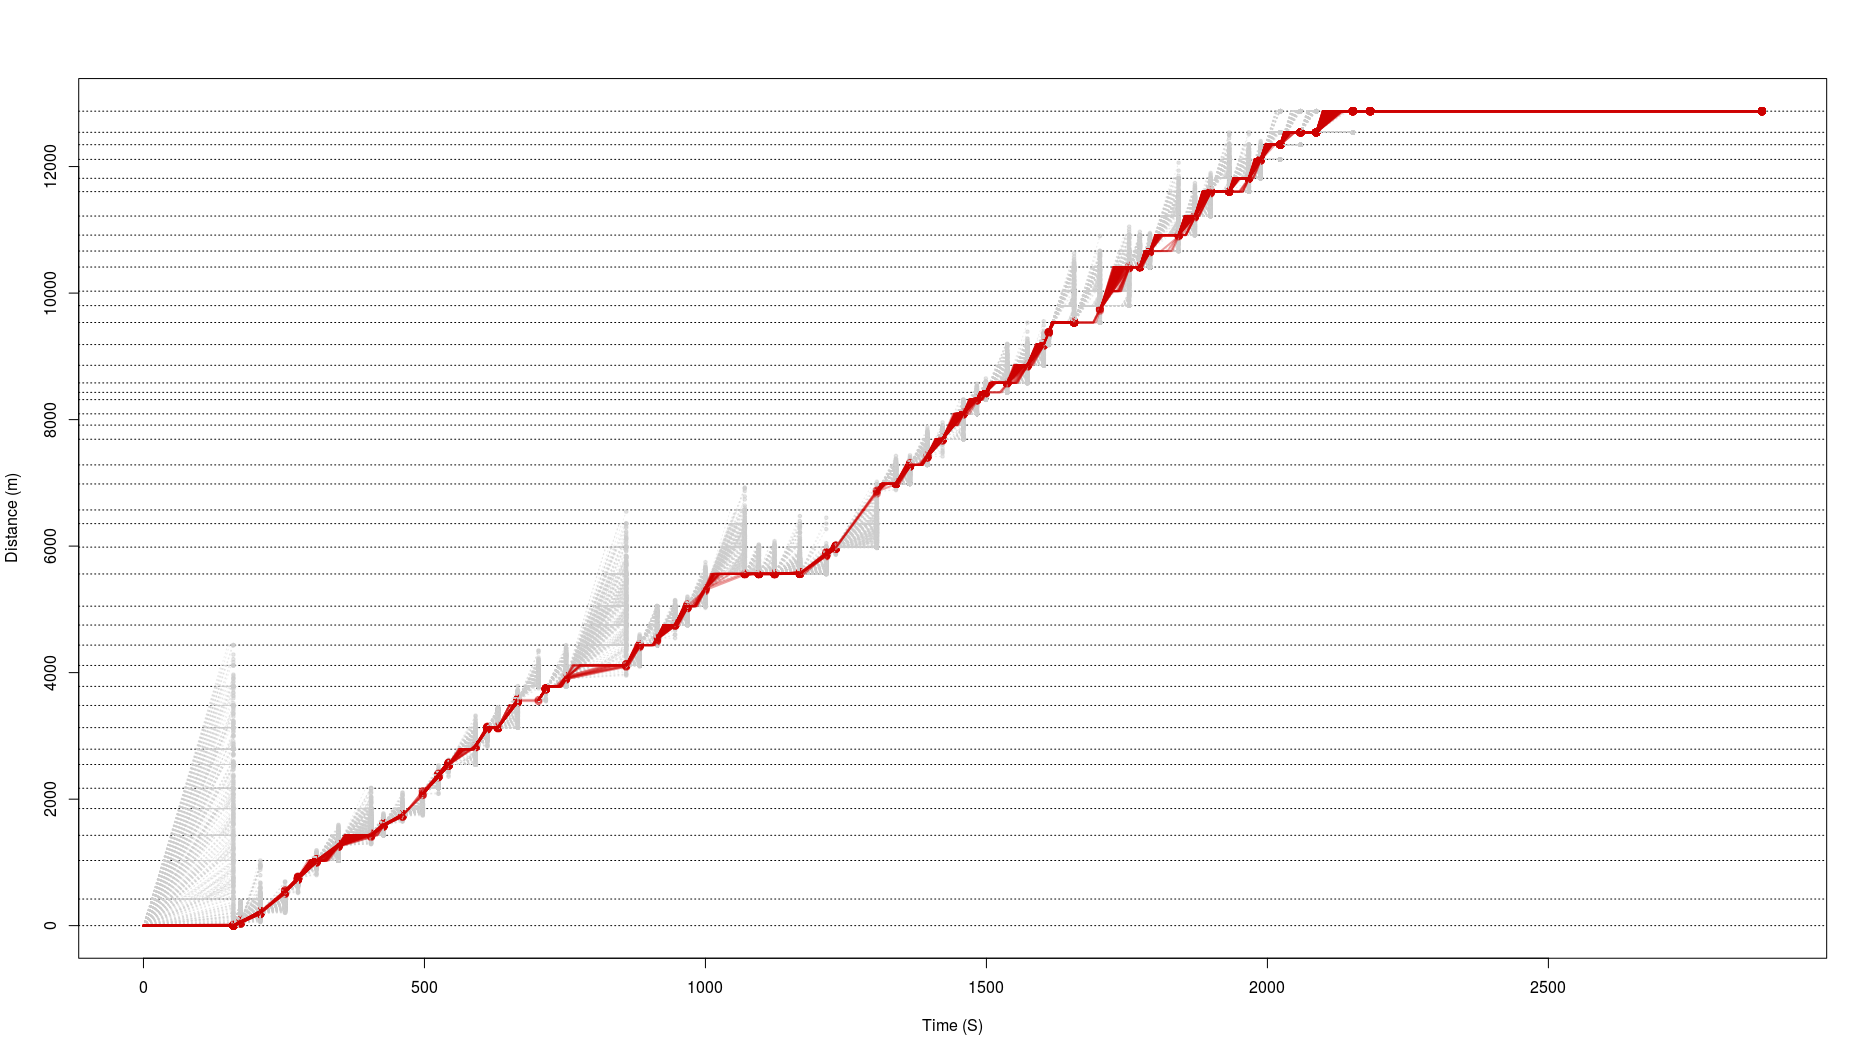
\includegraphics[width=\paperwidth]{figs/complete_route.png}
            };
        \end{tikzpicture}
     \end{frame}
}



\section{Predicting Arrival Times}

\begin{frame}{Predicting Arrival Times}
  \begin{itemize}
  \item each future stop along a route; up to 1~hour in advance
  \item prediction model needs to be far more precise than state model
  \item can be computationally complex
    \begin{itemize}
    \item over 1000 buses at peak times
    \item each with up to 10, 20, 30?? stops ahead
    \end{itemize}
  \end{itemize}

  %\item<2-> three examples:
  \onslide<2->
  \begin{exampleblock}{Three examples}
    \begin{enumerate}
    \item schedule
      
    \item historical data
      
    \item real-time data
    \end{enumerate}
  \end{exampleblock}
  %\end{itemize}
\end{frame}


\begin{frame}{Predicting Arrival Times: Schedule}
  \onslide<+->

  \begin{itemize}[<+- | alert@+>]
  \item each \emph{trip} has a \emph{schedule} with ``average'' arrival times
  \item given a particle's distance into trip
  \item compare to scheduled ``arrival time'' at that ``distance''
  \item compute scheduled travel time to a stop
  \end{itemize}

  \begin{overprint}
    \onslide<2>
    \centering
    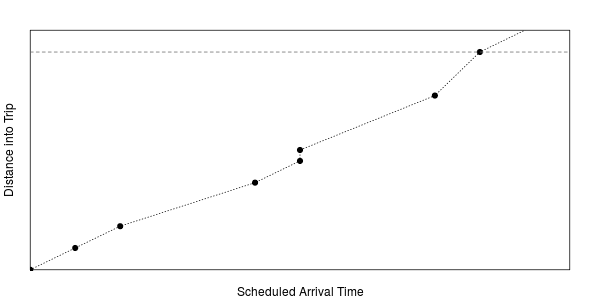
\includegraphics[width=0.8\textwidth]{figs/pred-sched-frame1.png}
    \onslide<3>
    \centering
    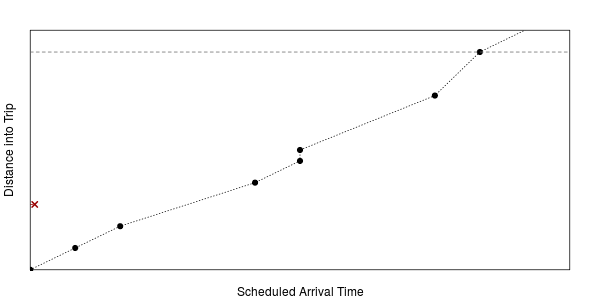
\includegraphics[width=0.8\textwidth]{figs/pred-sched-frame2.png}
    \onslide<4>
    \centering
    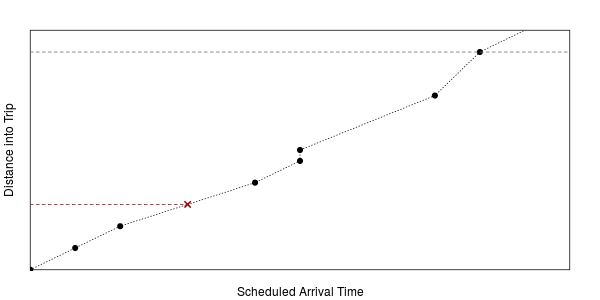
\includegraphics[width=0.8\textwidth]{figs/pred-sched-frame3.png}
    \onslide<5->
    \centering
    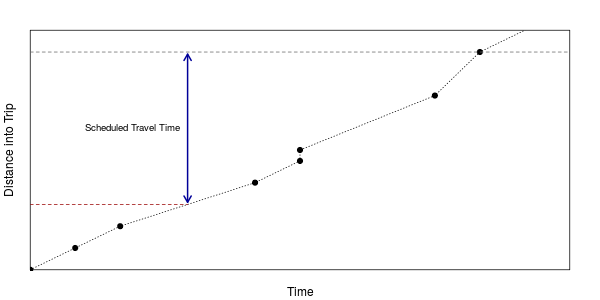
\includegraphics[width=0.8\textwidth]{figs/pred-sched-frame4.png}
  \end{overprint}

  \onslide<+->
\end{frame}


\begin{frame}{Predicting Arrival Times: Historical Data}
  \onslide<+->

  \begin{itemize}
  \item replace schedule times with \emph{historical times}
  \item can build up models (monotone regression?)\\
    covariates: day of the week, time of day, etc
  \item requires a lot of data (KNN, ANN, SVM, \ldots)\\
    \cite{mazloumi-etal:2011}: 6~months\\
    \cite{chen-rakha:2014}: 4~months \\
    \emph{For only a selection of test routes!}
  \item relies on patterns
  \end{itemize}
\end{frame}


\begin{frame}{Predicting Arrival Times: Real-time Data}  
  \begin{itemize}
  \item Real-time data for up to 1000+ Auckland buses available
  \item Particle Filter model provides distribution of speed at coordinates, $v_k$
  \item \cite{yu-etal:2011}: bus stops with multiple routes\\
    e.g., along Symonds St
  
    \vspace{1em}
  \item<2-> \textbf{Proposal}: combine travel times and speed estimates of \textbf{all} buses
    \begin{itemize}
    \item most up to date traffic/congestion data
    \item no extensive data collection, storage required
    \end{itemize}
  \end{itemize}
\end{frame}


{ % all template changes are local to this group.
    \setbeamercolor{background canvas}{bg=white}
\begin{frame}{Example (single route)}
  Bus Route 274, Three Kings to Britomart


  \begin{overprint}
    \onslide<1>
    \centering
    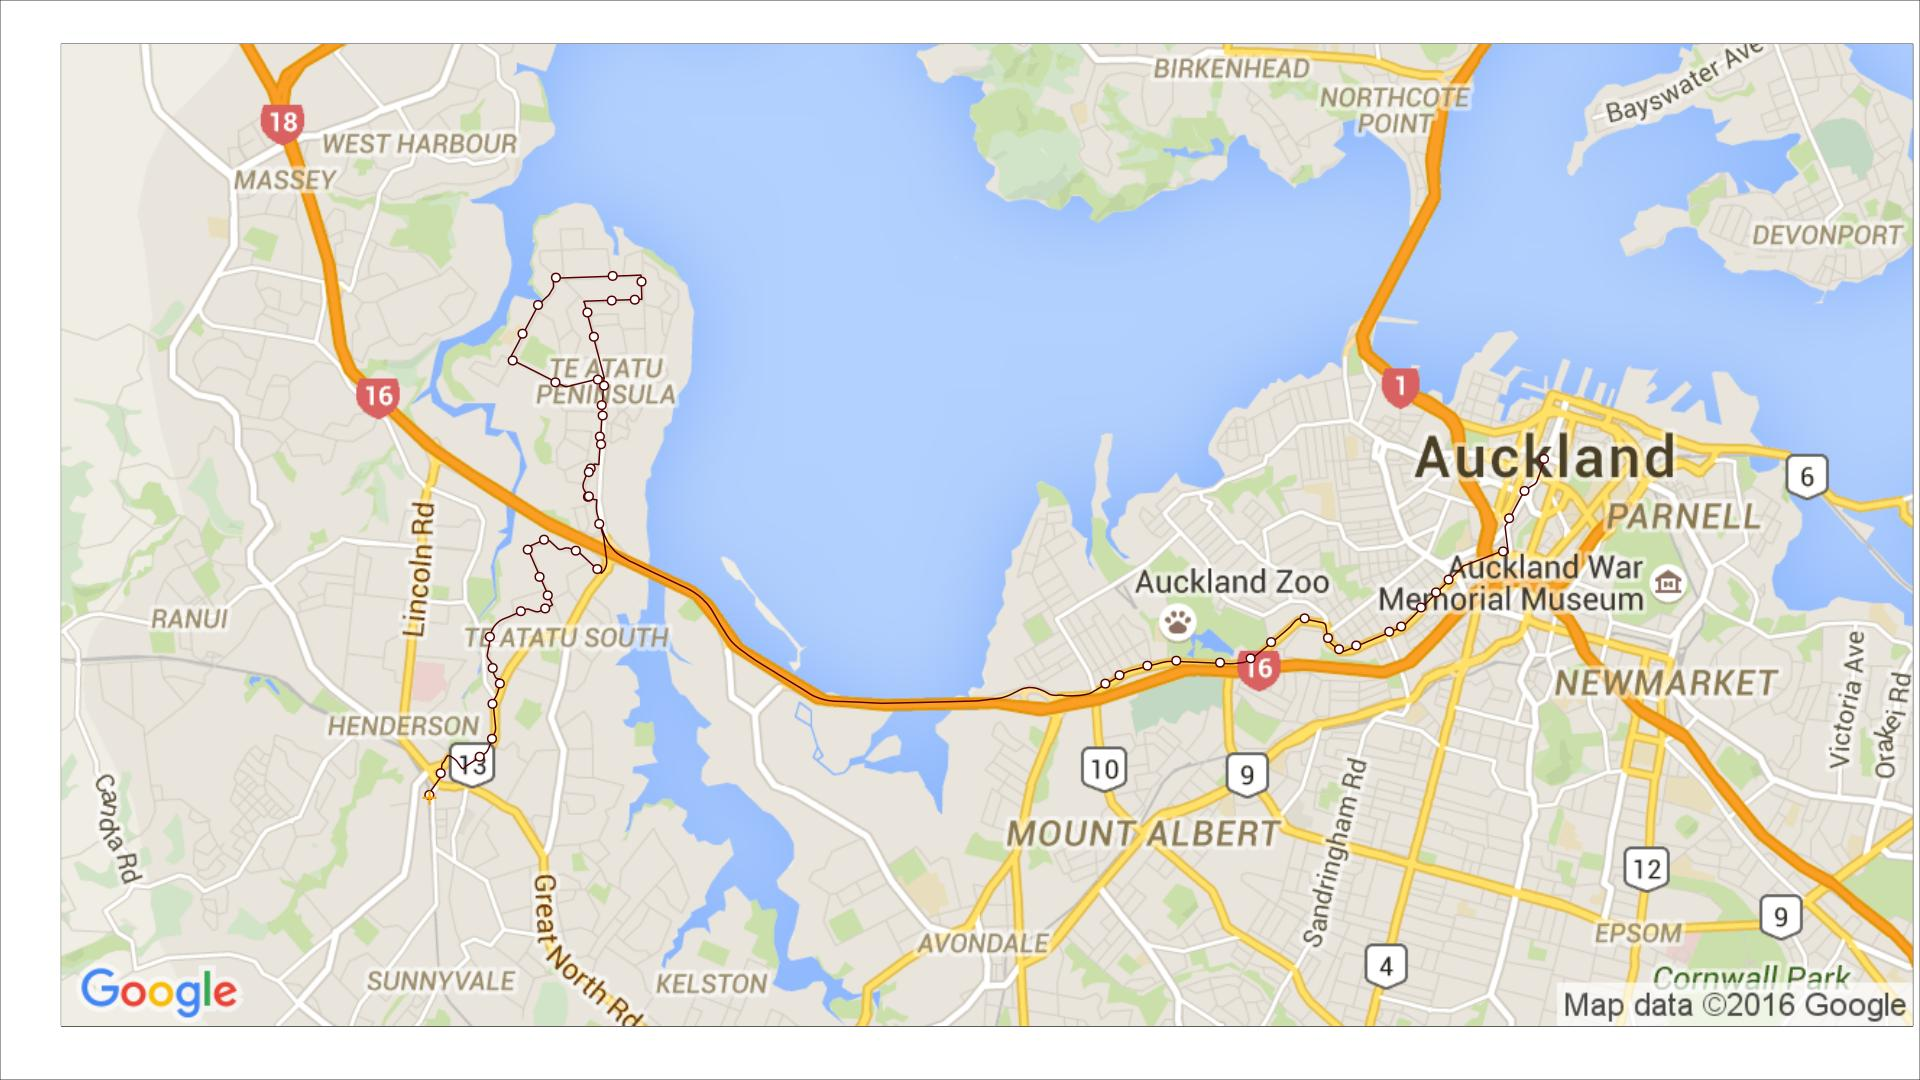
\includegraphics[width=1\textwidth]{figs/r274/TRIP5/particle_map001.jpg}

    \onslide<2>
    \vspace{2em}
    Particle Filter State Estimates and Transitions, 7am trip
    \centering
    \includegraphics[width=1\textwidth]{figs/r274/TRIP5/distance_traveled.jpg}

    \onslide<3>
    \vspace{2em}
    ``Historical'' Data, 5:30am, 6:00am, 6.30am, 6:50am
    \centering
    \includegraphics[width=0.45\textwidth]{figs/r274/TRIP1/distance_traveled.jpg}
    \includegraphics[width=0.45\textwidth]{figs/r274/TRIP2/distance_traveled.jpg}\\
    \includegraphics[width=0.45\textwidth]{figs/r274/TRIP3/distance_traveled.jpg}
    \includegraphics[width=0.45\textwidth]{figs/r274/TRIP4/distance_traveled.jpg}

    \onslide<4>
    \vspace{2em}
    Arrival time prediction based on 4 previous trips (averaged)
    \centering
    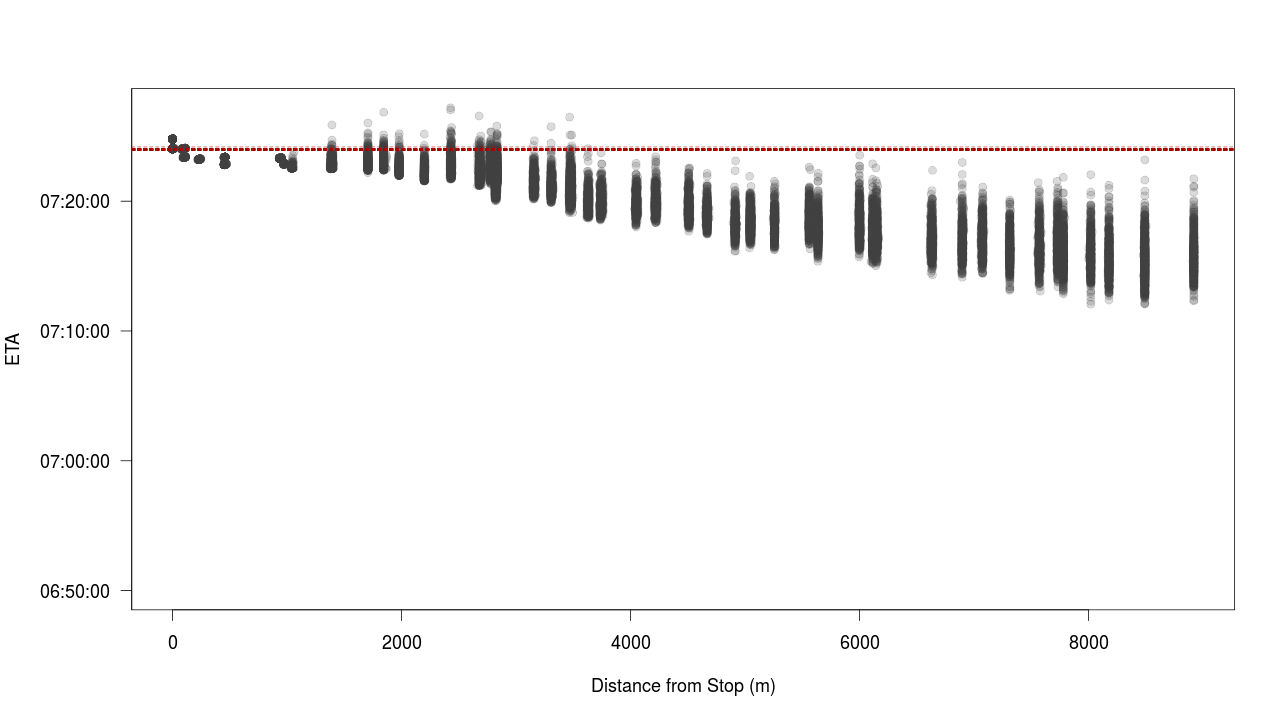
\includegraphics[width=1\textwidth]{figs/r274/TRIP5/arrival_last_hist.jpg}
  \end{overprint}
\end{frame}
}


\section{Making Predictions Accessible}

\begin{frame}{Communicating Predictions}
  \onslide<+->

  \begin{itemize}[<+->]

  \item target audience: \emph{general public}
    
  \item significant uncertainty in predictions

  \item how to convey \emph{distribution of particles}, uncertainty?

  \item \textbf{point estimates}:
    \begin{itemize}[<1->]
    \item good for displays that can only fit a single digit
    \item for commuters, they imply ``accuracy''
    \end{itemize}
    
  \item \textbf{interval estimates}:
    \begin{itemize}[<1->]
    \item standard practice for most statistical analyses
    \item \emph{meaningful} interval for commuters?\\
      i.e., ETA: 3--7~mins = BETWEEN 3 and 7 minutes?
    \item non-symmetrical interval for journey planning:\\
      bus arriving later (8~min) better than earlier (2~min)!
    \end{itemize}
  \end{itemize}

\end{frame}



\begin{frame}{Journey Planning}
  \begin{itemize}[<+->]
  \item \alert<5->{``I want to travel from A to B \ldots}
    \begin{itemize}
    \item \alert<5>{``\ldots leaving whenever, by the fastest route.''}
    \item \alert<6>{``\ldots and arrive ASAP.''}
    \item \alert<7>{``\ldots and arrive before 8am.''}
    \end{itemize}
  \end{itemize}
  
  \vspace{1em}
  \metroset{block=fill}
  \begin{overprint}
    \onslide<5>
    \begin{block}{Fastest route}
      \begin{itemize}
      \item If there are multiple routes, which is fastest?
      \item What time should I be at the stop by to minimise wait time, but not miss the
        bus?
      \end{itemize}
    \end{block}
    \onslide<6>
    \begin{block}{Arrive ASAP}
      \begin{itemize}
      \item Which bus from A will arrive at B soonest
      \item that hasn't left yet/by the time I get to the bus stop
      \end{itemize}
    \end{block}
    \onslide<7>
    \begin{block}{Arrive on time}
      \begin{itemize}
      \item If there are multiple routes, which will get there on time?
      \item Without being \emph{too} early?
      \item Which is most reliable?
      \end{itemize}
    \end{block}
  \end{overprint}
\end{frame}


\begin{frame}{References}
  \scriptsize
  \begingroup
  \renewcommand{\section}[2]{}%
  \bibliographystyle{./elsart-harv} % elsart-harv,plain,unsrt,alpha
  \bibliography{./myrefs}
  \endgroup
\end{frame}



\begin{frame}[standout]
  Thank you!
\end{frame}


\end{document}
